\capitulo{5}{Aspectos relevantes del desarrollo del proyecto}

Este proyecto de investigación pretende abarcar tanto la parte más teórica de algunos de los algoritmos más relevantes de aprendizaje semisupervisado, como su aplicación en diversos ámbitos de la ciberseguridad. Por ello, en este apartado se pueden encontrar diversos puntos importantes.

En la primera subsección~\ref{sec:5_ssl} se desarrollará cómo se han validado los algoritmos de aprendizaje implementados. Para ello, se definirá qué experimentos se han realizado, se reportarán los resultados obtenidos y se realizarán comparativas contra otras implementaciones.

En la segunda subsección~\ref{sec:5_detec_ataques} se mostrarán los resultados obtenidos tras aplicar métodos de aprendizaje a la detección de ataques en sistemas de recomendación y se valorará si el método de generación de vectores de características expuesto en~\ref{sec:vectores_catacterísticas_ataquesisrec} es extrapolable a una aplicación real.

Por último, en la tercera subsección~\ref{sec:5_phishing} (dedicada al \textit{phishing}), se estudiarán los resultados del método de extracción expuesto en~\ref{sec:vectores_caracteristicas_phishing}.

\section{Algoritmos de aprendizaje semisupervisado}
\label{sec:5_ssl}

Uno de los principales objetivos del proyecto es entender e implementar (siendo capaz de tomar decisiones de implementación no arbitrarias en caso de que sea requerido) algunos de los algoritmos de aprendizaje semisupervisado más relevantes. Además, se ha querido ser crítico con estos métodos, y para ello se ha buscado validar su funcionamiento mediante diversos experimentos.

A continuación se facilitan los resultados de las pruebas realizadas con las implementaciones propias de algunos métodos de aprendizaje semisupervisado. Para evaluar la calidad de las implementaciones, se han utilizado algunos de los \textit{dataset} más comunes en métodos de clasificación. En concreto, se han utilizado los que están disponibles en la librería Scikit-learn, que se muestran en la tabla~\ref{tabla_datasets_sklearn}. El parámetro $n$ representa el número de instancias que contiene un determinado conjunto de datos, mientras que el parámetro $m$ muestra el número de características que contiene cada una de esas instancias.

\begin{table}
	\small
	\begin{centering}
		\begin{tabular}{@{}p{4em} p{20em} r r r @{}}
			\toprule
			\textbf{Nombre} & \textbf{Descripción} & \textbf{Clases} & $n$ & $m$\\ 
			\midrule
			
			Iris & Conjunto de instancias pertenecientes a diferentes tipos de plantas de la especie Iris. & 3 & 150 & 4 \\\\
			Dígitos & Conjunto de instancias que representan una imagen de 8x8 perteneciente a un dígito. & 10 & 1797 & 64 \\\\
			Vino & Conjunto de instancias pertenecientes a tres clases de vino con sus parámetros estimados mediante análisis químico. & 3 & 178 & 13 \\\\
			Cáncer de Mama & Conjunto de instancias que representan parámetros de distintas mujeres que pueden padecer o no cáncer (clasificación binaria). & 2 & 569 & 30 \\
			\bottomrule
		\end{tabular}
	\end{centering}
	\caption[Experimentación: \textit{datasets} estándar]{Descripción de los \textit{datasets} utilizados para validar los algoritmos.}
	\label{tabla_datasets_sklearn}	
\end{table}



\subsection{Co-forest}

Para comprobar la correctitud del algoritmo se han realizado diversos experimentos. En primer lugar, se ha evaluado el modelo en diversas situaciones de su ciclo de vida. Posteriormente, se ha realizado una comparativa contra la implementación proporcionada por KEEL.

\subsubsection{Experimentación con el algoritmo}

Los resultados se pueden observar en las gráficas~\ref{gr:cf_train-iterations},~\ref{cf:cf_time-percentage} y ~\ref{cf:tt_trees}.


\begin{itemize}
	\item \textbf{Fase de entrenamiento:} como se ha desarrollado en los conceptos teóricos, la fase de entrenamiento en el \textit{co-forest} es iterativa, y finaliza cuando ningún árbol recibe nuevas pseudo-etiquetas que puedan cambiar su comportamiento (en la fase de re-entrenamiento).
	
	Se ha querido estudiar la evolución del \textit{score} (porcentaje de aciertos respecto al total de las predicciones) del algoritmo durante la fase de entrenamiento para los cuatro conjuntos de datos definidos en la tabla~\ref{tabla_datasets_sklearn}. Para ello, se ha realizado una gráfica ilustrando cómo evoluciona en función de la iteración en la que se encuentre.
	
	\begin{figure}[h]
		\caption[\textit{Co-Forest}: distribución de datos entrenamiento y \textit{test}]{Gráfica que representa la distribución de los datos.}
		\centering
		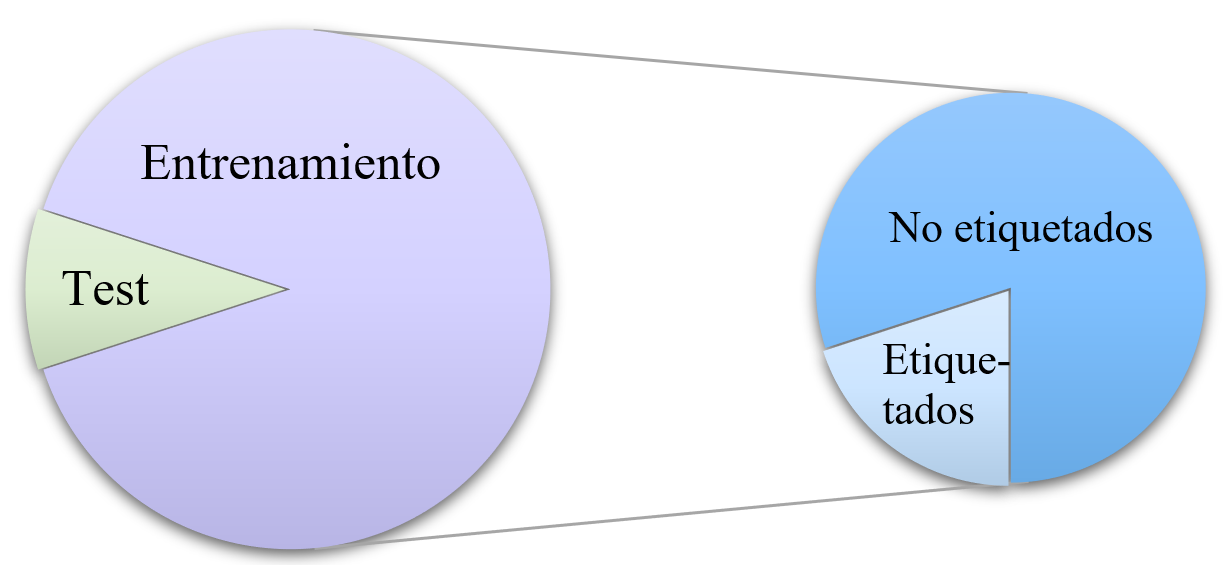
\includegraphics[scale=0.3]{../img/memoria/5_entrenamiento_particiones}
		\label{5_entrenamiento_particiones}
	\end{figure}

	Para garantizar que los resultados obtenidos no son producto de una partición concreta de los datos, se ha realizado validación cruzada (con 10 particiones sin repetición). Por lo tanto, el porcentaje de datos utilizados para el entrenamiento es el $90\%$ del total (utilizando estratificación). Los datos de entrenamiento, a su vez, se dividen en etiquetados y no etiquetados. En este caso, el $20\%$ representa los datos etiquetados, y el $80\%$ los no etiquetados, como se puede observar en la imagen~\ref{5_entrenamiento_particiones}. Se han utilizado 20 árboles.
	
	La exactitud media obtenida se puede ver representada en la gráfica~\ref{gr:cf_train-iterations}. Es destacable que, dependiendo de los datos que se utilicen para entrenar el \textit{co-forest}, puede variar el número de iteraciones que se necesiten (incluso dentro de un mismo \textit{dataset}). Por ello, siempre se representa el número máximo de iteraciones realizadas, y para no deformar la media, se ha considerado que el valor de las iteraciones inexistentes es el mismo que el valor obtenido en la última iteración (ya que si, el algoritmo siguiese, el resultado devuelto sería igual debido a que no se volvería a entrenar ningún árbol).
	
	\begin{figure}[h]
		\caption[\textit{Co-Forest}: resultados (iteraciones-entrenamiento)]{Gráfica que muestra la evolución de la \textit{accuracy} para cada \textit{dataset} (además de su desviación) durante las iteraciones del entrenamiento del \textit{co-forest}.}
		\centering
		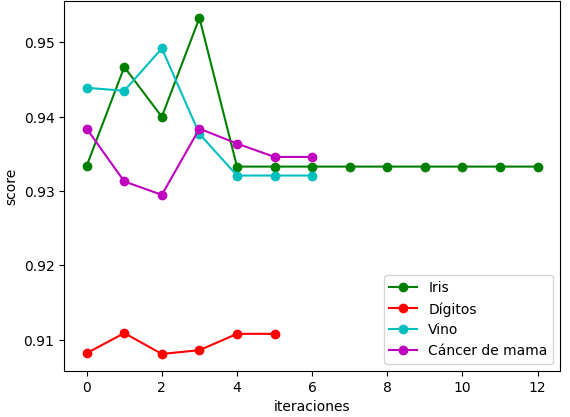
\includegraphics[scale=0.55]{../img/memoria/5_coforest_score-iteraciones}
		\label{gr:cf_train-iterations}
	\end{figure}

	Como se puede comprobar, el modelo mejora los resultados iniciales (exactitud obtenida en la iteración $0$, cuando todavía no se ha realizado entrenamiento semi-supervisado y se cuenta con un \textit{random forest} tradicional) en dos de los conjuntos de datos, mientras que en los otros dos empeora. Este comportamiento es lógico debido a que no todos los modelos son apropiados para todos los conjuntos de datos. Si se observa con más detenimiento cada conjunto de datos individualmente en el resto de los cuadrantes de la gráfica~\ref{gr:cf_train-iterations}, se puede observar que la desviación típica varía considerablemente, por lo que se puede deducir que el modelo podría llegar a ser utilizable en la mayoría de los casos si la partición es la adecuada.

	\item \textbf{Tiempo de entrenamiento:} además, también se ha querido evaluar cómo varía el tiempo de entrenamiento en función del número de instancias utilizadas. Para ello, se ha trabajado con el \textit{dataset} que contiene un mayor número de datos (Dígitos), y los resultados obtenidos se pueden observar en el primer cuadrante de la gráfica~\ref{cf:cf_time-percentage}. Como se puede comprobar, sigue un crecimiento aproximadamente lineal. La velocidad, en este caso, es alta, pero cabe recordar que depende en gran medida del número de árboles utilizados y de las iteraciones que estos realicen. Se ha representado en la línea negra punteada, además, el resultado del modelo de regresión lineal.

\begin{figure}[h]
	\caption[\textit{Co-Forest}: resultados (tiempo-porcentaje)]{Gráfica que muestra el tiempo de entrenamiento requerido para el \textit{co-forest} en función del número de instancias, además de la evolución del \textit{score} (\textit{accuracy}) en función del porcentaje total de datos destinado al entrenamiento.}
	\centering
	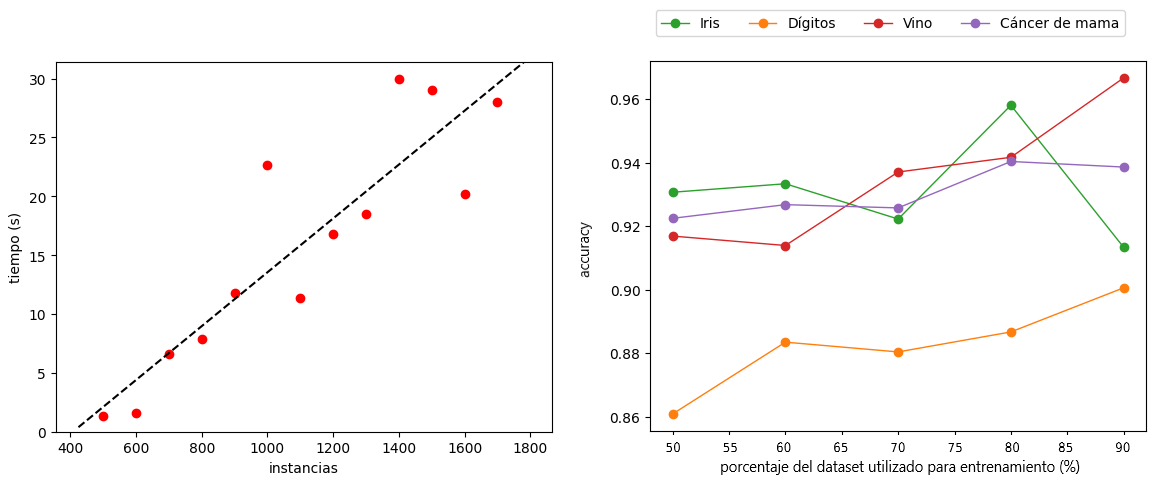
\includegraphics[scale=0.4]{../img/memoria/5_coforest_time-percentage}
	\label{cf:cf_time-percentage}
\end{figure}


	\item \textbf{Datos de entrenamiento:} En este apartado de la experimentación, se ha querido evaluar cómo se comporta el \textit{co-forest} en función del porcentaje de datos que se utilice para el entrenamiento. Nuevamente, se han utilizado  $20$ árboles, y la división del conjunto de datos de entrenamiento se ha mantenido: $20\%$ etiquetados y $80\%$ no etiquetados. Los conjuntos están estratificados.
	
	Como se puede comprobar en el segundo cuadrante de la gráfica~\ref{cf:cf_time-percentage}, sigue el comportamiento esperado, y por lo general a más instancias utilizadas para entrenar el modelo, mejor desempeño presenta. Nuevamente, recalcar que el resultado obtenido es la media de 10 experimentos realizados.
	
	\item{\textbf{Número de árboles}}: Hasta este momento, todos los resultados han sido realizados para $n=20$. Es decir, utilizando $20$ árboles. Sin embargo, el comportamiento del \textit{co-forest} varía considerablemente en función del número de árboles contenidos en el \textit{ensemble}, lo que motiva la realización del siguiente experimento. Nuevamente, se ha desarrollado utilizando cuatro conjuntos de datos y validación cruzada, por lo que se muestra la media en la exactitud para las $10$ particiones.
	
	Como se puede comprobar en la gráfica~\ref{cf:tt_trees}, en general, cuantos más árboles se utilicen, mejor \textit{score} alcanza el \textit{co-forest}. Es destacable que, evidentemente, a mayor $n$, mayor tiempo de procesamiento es requerido, como se ilustra en el segundo cuadrante de esa misma gráfica. Por lo tanto, se debería alcanzar un compromiso. Por lo general, los autores~\cite{originalCoForest2007} utilizan valores de $n \geq 6$.
	
	\begin{figure}[h]
		\caption[\textit{Co-Forest}: resultados (número de árboles)]{Gráfica que muestra la \textit{accuracy} alcanzada por el \textit{co-forest}, además del tiempo de entrenamiento requerido en función del número de árboles utilizados}
		\centering
		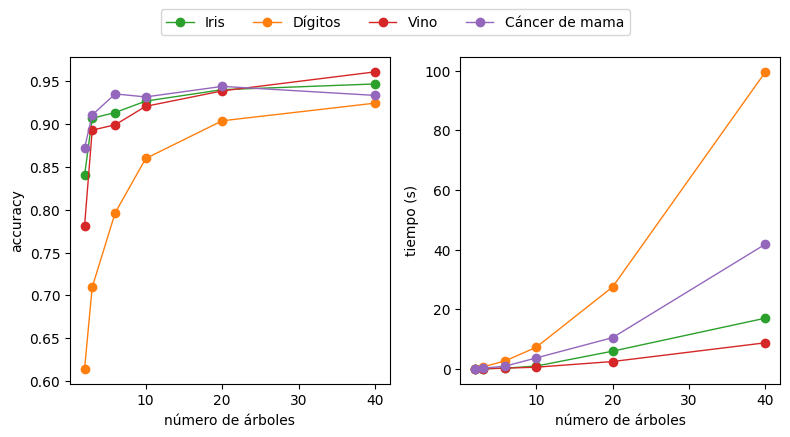
\includegraphics[scale=0.7]{../img/memoria/5_coforest_trees}
		\label{cf:tt_trees}
	\end{figure}
	
\end{itemize} 


\subsubsection{Comparativa contra KEEL}

Para asegurar el correcto funcionamiento del algoritmo implementado, se ha decidido comparar contra la herramienta KEEL, creada por distintas universidades españolas y financiada por el Ministerio de Educación y Ciencia.

En primer lugar y para tener más capacidad de <<manipulación>>, se optó por descargar los ficheros fuentes de la última versión de Github~\cite{keelRepo} en lugar de utilizar la versión compilada que ofrecen los desarrolladores. Se puede consultar cómo en los anexos.

Para comparar los algoritmos en las condiciones más realistas posibles, se definieron las características mostradas en la tabla~\ref{tabla_coforest_keelvsnuestro_diseño}.

\begin{table}
	\begin{centering}
		\begin{tabular}{@{}p{10em} p{20em} @{}}
			\toprule
			\textbf{Parámetro} & \textbf{Valor} \\ 
			\midrule
			$n$ & 6\\
			$\theta$ & 0.75 \\
			\textit{Folds} & 10 \\
			\% etiquetados & 10\% (en el conjunto de entrenamiento). \\
			Comentarios & Para la comparativa se han utilizado los \textit{datasets} Iris y Vino, ambos estratificados.\\
			\bottomrule
			
		\end{tabular}
	\end{centering}
	\caption[\textit{Co-forest}: resumen del experimento]{Tabla resumen con el diseño del experimento.}
	\label{tabla_coforest_keelvsnuestro_diseño}	
\end{table}

\begin{table}
	\begin{centering}
		
		\begin{tabular}{@{} p{4em} p{5em} p{7em} p{7em} p{7em} @{}}
			\toprule
			\multirow{2}{*}{\textbf{\textit{ \hfil Fold}}} & \multicolumn{2}{c}{\hfil \textbf{Iris}}& \multicolumn{2}{c}{\hfil \textbf{Vino}} \\
			\cmidrule{2-3} \cmidrule{4-5}
			& \hfil Propia & \hfil KEEL & \hfil Propia & \hfil KEEL\\ 
			\toprule
			\hfil 1 &\hfil 1.00	&\hfil 0.87	& \hfil 0.89  & \hfil0.83 \\
			\hfil 2 &\hfil 0.86	&\hfil 0.80	& \hfil 1.00 	&  \hfil 0.94 \\
			\hfil 3 & \hfil 1.00	& \hfil 1.00	& \hfil 0.94	& \hfil 1.00 \\
			\hfil 4 & \hfil 1.00	& \hfil 1.00	& \hfil 0.94	& \hfil 0.89 \\
			\hfil 5 & \hfil 0.87	& \hfil 1.00	& \hfil 0.65	& \hfil 0.88 \\
			\hfil 6 & \hfil 0.93	& \hfil 0.93	& \hfil 0.94	& \hfil 0.71 \\
			\hfil 7 & \hfil 0.93	& \hfil 1.00	& \hfil 0.83	& \hfil 0.89 \\
			\hfil 8 & \hfil 0.93	& \hfil 0.93	& \hfil 0.94	& \hfil 0.78 \\
			\hfil 	9 & \hfil 0.93	& \hfil 0.93	& \hfil 0.67	& \hfil 0.72 \\
			\hfil 10& \hfil 0.87	& \hfil 0.87	& \hfil 0.94	& \hfil 0.94 \\
			\midrule
			\hfil \textbf{Media} 			& \hfil 0.93	& \hfil 0.93	& \hfil 0.88	& \hfil 0.86 \\
			\bottomrule
		\end{tabular}
	\end{centering}
	\caption[\textit{Co-forest}: comparativa entre KEEL y la implementación propia]{Comparativa entre la \textit{accuracy} del \textit{co-forest} de KEEL y la implementación propia sobre el conjunto de \textit{test}.}
	\label{tabla_coforest_keelvsnuestro}	
\end{table}

Dentro de los ficheros fuente de KEEL, se pueden encontrar distintos conjuntos de datos con las particiones del \textit{k-cross-validation} ya hechas y que son utilizadas en las ejecuciones de sus experimentos. Para comprobar ambos algoritmos en igualdad de condiciones, se convirtieron dichos archivos \texttt{*.dat} en \texttt{*.csv} y se importaron en la implementación propia mediante la librería Pandas. De esta manera, el único parámetro que no es idéntico entre ambas implementaciones es qué instancias de entre los datos etiquetados seleccionan los árboles para entrenarse en un primer momento (son aleatorios y generar las pequeñas diferencias observadas).

Los resultados obtenidos se pueden observar en la tabla~\ref{tabla_coforest_keelvsnuestro}. Como se puede comprobar, ambos algoritmos obtienen resultados prácticamente idénticos, siendo un poco superior el porcentaje de acierto logrado por la herramienta implementada propia en el caso del \textit{dataset} Vino.


\subsection{Tri-Training}

Al igual que en los algoritmos anteriores, se ha decidido experimentar con distintas opciones a la hora de representar las gráficas, además de realizar una comparativa contra sslearn y LAMDA para probar la implementación.


\subsubsection{Experimentación con el algoritmo}

Los resultados se pueden observar en las gráficas~\ref{gr:tt_train-iterations} y~\ref{gr:tt_time-percentage}.

\begin{figure}[h]
	\caption[\textit{Tri-training}: resultados (iteraciones-entrenamiento)]{Gráfica que muestra la evolución de la \textit{accuracy} para cada \textit{dataset} (además de su desviación) durante las iteraciones del entrenamiento del \textit{tri-training}.}
	\centering
	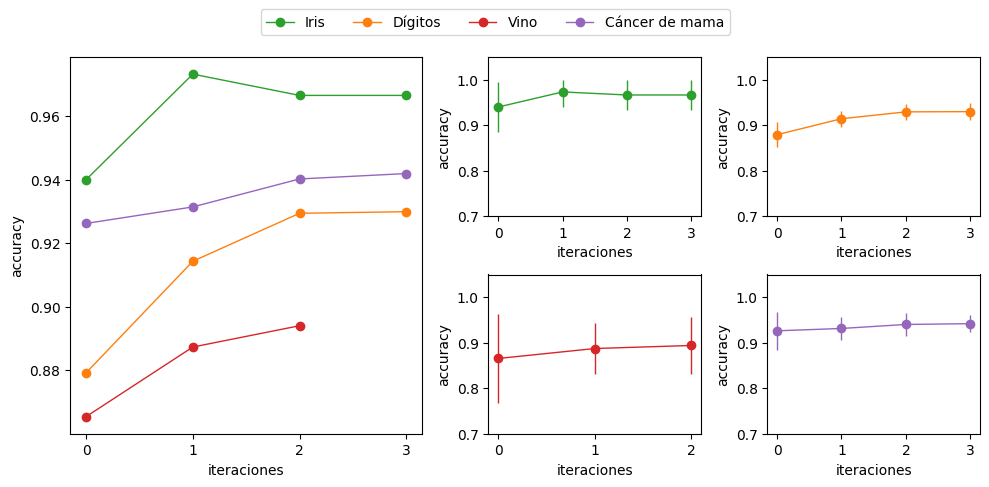
\includegraphics[scale=0.5]{../img/memoria/5_tritraining_score-iteraciones}
	\label{gr:tt_train-iterations}
\end{figure}

\begin{figure}[h]
	\caption[\textit{Tri-training}: resultados (tiempo-porcentaje)]{Gráfica que muestra el tiempo de entrenamiento requerido para el \textit{tri-training}, además de la evolución del \textit{score} en función del número de instancias.}
	\centering
	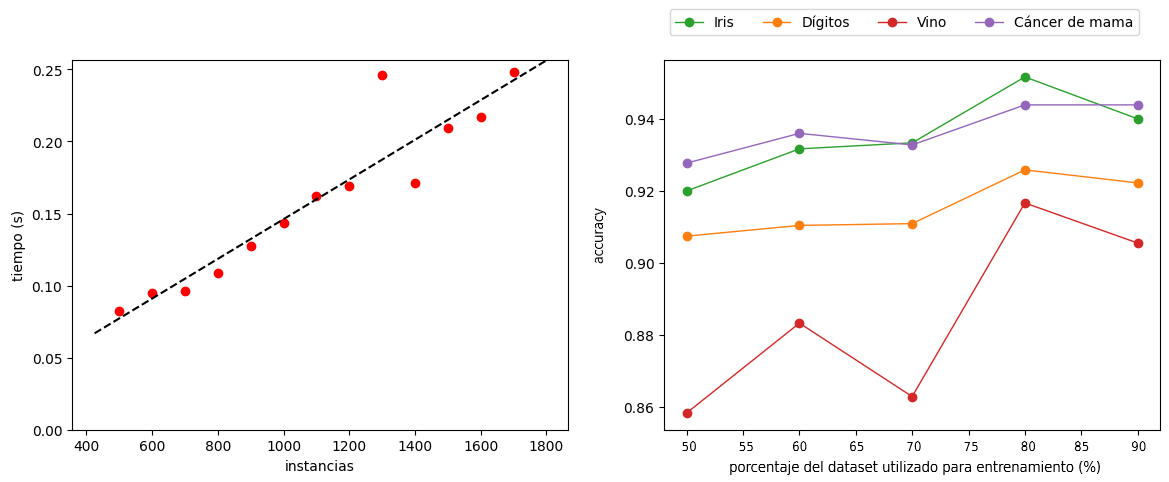
\includegraphics[scale=0.4]{../img/memoria/5_tritraining_time-percentage}
	\label{gr:tt_time-percentage}
\end{figure}

\begin{itemize}
	\item \textbf{Fase de entrenamiento:} se ha querido evaluar la evolución de la \textit{accuracy} del modelo en función de la iteración del entrenamiento en la que se encuentre. En este caso, el \textit{tri-training} utiliza como estimadores base un \textit{naive-bayes} gaussiano, un árbol de decisión y un \textit{$k$NN}. Al igual que en el \textit{co-forest}, los resultados representados son la media de 10 experimentos realizados mediante validación cruzada (10 <<entrenamientos>> distintos) y se pueden observar en la gráfica~\ref{gr:tt_train-iterations}, donde el primer cuadrante compara todos los \textit{datasets} y el resto representa la desviación entre las distintas fases de entenamiento para cada \textit{dataset}.
	
	Como se puede comprobar, el modelo mejora los resultados iniciales (exactitud obtenida en la iteración $0$, cuando todavía no se ha comenzado el algoritmo de entrenamiento semisupervisado), siendo especialmente notable en los \textit{datasets} Vino y Dígitos. Por ello, se deduce que la incorporación del conjunto de datos no etiquetado durante el entrenamiento es útil y mejora la hipótesis aprendida en cada uno de los clasificadores base (y, por ello, la general del \textit{ensemble}).
	
	\item \textbf{Tiempo de entrenamiento:} nuevamente se ha trabajado con el \textit{dataset} que contiene un mayor número de datos y los resultados obtenidos se representan en el primer cuadrante de la gráfica~\ref{gr:tt_time-percentage}. Como se puede observar, el tiempo crece de forma aproximadamente lineal con una alta velocidad (debido en parte a que este \textit{dataset} no realiza un número elevado de iteraciones durante el entrenamiento).
	
	\item \textbf{Datos de entrenamiento:} en este caso, se quiere evaluar el desempeño del \textit{tri-training} en función del porcentaje del \textit{dataset} que se utilice para el entrenamiento (posteriormente este conjunto será dividido en $L$ ($20\%$) y $U$ ($80\%$)). Los resultados mostrados son la media de 10 experimentos y se observan en el segundo cuadrante de la gráfica~\ref{gr:tt_time-percentage}. En este caso, un buen compromiso sería utilizar un $80\%$ de los datos, ya que por lo general a mayor número de instancias utilizadas durante el entrenamiento mejor resultado, no alcanzándose siempre la máxima exactitud cuando se usa el mayor porcentaje.
\end{itemize} 

\subsubsection{Comparativa contra sslearn y LAMDA}

En el caso del \textit{tri-training}, existen implementaciones en Python que, además, permiten que los estimadores base utilizados sean los disponibles en la librería Scikit-learn. Estas son sslearn, biblioteca de aprendizaje semisupervisado escrita por José Luis Garrido-Labrador y disponible en Github~\cite{sslearnRepo} y LAMDA, un \textit{toolkit}~\cite{lamdasslPaper} desarrollado por Lin-Han Jia (y su equipo) que se encuentra públicamente disponible para su uso~\cite{lamdasslRepo}.

Para la comparativa se ha realizado validación cruzada utilizando 10 \textit{folds}. Evidentemente, ambos modelos han sido entrenados con el mismo conjunto de entrenamiento (más concretamente, idénticos $L$ y $U$) y probados con el mismo conjunto de \textit{test}. Como estimadores base se ha utilizado el árbol de decisión disponible en la librería Scikit-learn.

\begin{figure}[h]
	\caption[\textit{Tri-training}: comparativa contra LAMDA]{Gráfica que representa la variación de la \textit{accuracy} en cada \textit{fold} y la media para la implementación del \textit{tri-training} de LAMDA y la propia.}
	\centering
	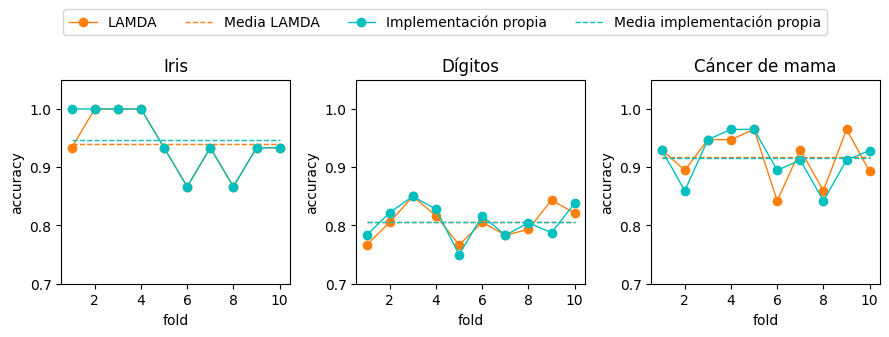
\includegraphics[scale=0.62]{../img/memoria/5_tritraining_lamda}
	\label{gr:tt_vs_lamda}
\end{figure}

En el caso de la comparativa contra \textit{sslearn}, el resultado se puede contemplar en la gráfica~\ref{gr:tt_vs_sslearn}, mientras que el caso de LAMDA se observa en la gráfica~\ref{gr:tt_vs_lamda}. Como se puede comprobar, la media de la \textit{accuracy} para ambos modelos es prácticamente idéntica. Hay algunas variaciones en la \textit{score} para distintos \textit{folds}, pero pueden deberse a detalles de implementación y selección de los conjuntos internamente. Por este motivo, la implementación se considera correcta.

\begin{figure}[h]
	\caption[\textit{Tri-training}: comparativa contra \textit{sslearn}]{Gráfica que representa la variación de la \textit{accuracy} en cada \textit{fold} y la media para la implementación del \textit{tri-training} de \textit{sslearn} y la propia.}
	\centering
	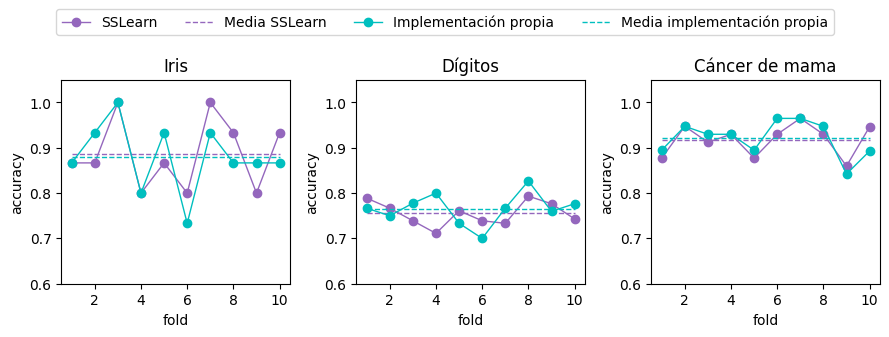
\includegraphics[scale=0.62]{../img/memoria/5_tritraining_sslearn}
	\label{gr:tt_vs_sslearn}
\end{figure}


\subsection{Democratic-co Learning}

En este algoritmo se facilitan las mismas experimentaciones previas, además de una comparativa contra sslearn~\cite{sslearnRepo}.

\subsubsection{Experimentación con el algoritmo}
Los resultados se pueden observar en las gráficas~\ref{gr:dc_train-iterations} y~\ref{gr:dc_time-percentage}.

\begin{figure}[h]
	\caption[\textit{Democratic-co}: resultados (iteraciones-entrenamiento)]{Evolución de la \textit{accuracy} para cada conjunto de datos y representación (para cada \textit{dataset}) de la desviación estándar durante las iteraciones del entrenamiento del \textit{democratic-co learning}.}
	\centering
	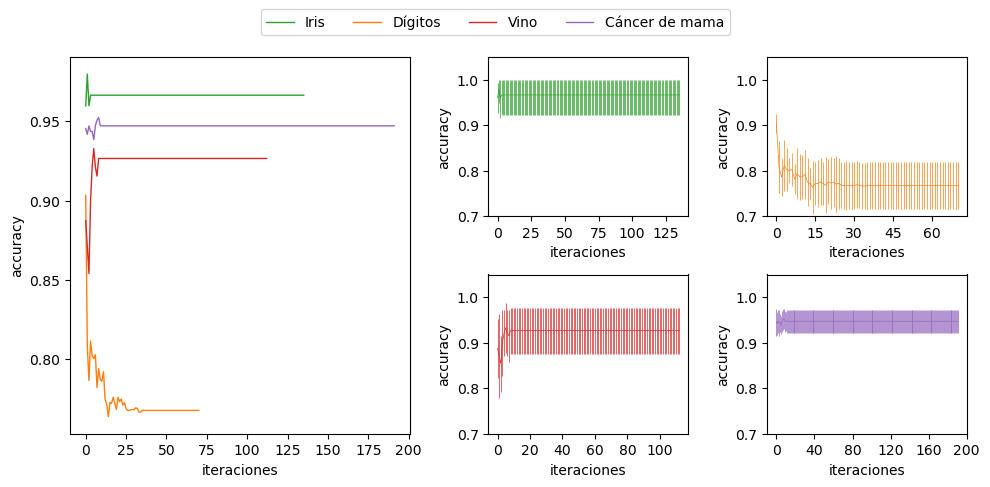
\includegraphics[scale=0.5]{../img/memoria/5_democraticco_score-iteraciones}
	\label{gr:dc_train-iterations}
\end{figure}

\begin{itemize}
	\item \textbf{Fase de entrenamiento:} como estimadores base para el \textit{democratic-co learning} se han utilizado un \textit{naive-bayes} gaussiano, un árbol de decisión y un \textit{$k$NN} con $n = 3$. Nuevamente, los resultados representados han sido obtenidos mediante validación cruzada y se representan en la gráfica~\ref{gr:dc_train-iterations}.
	
	Como se puede observar, todos los \textit{datasets} mejoran la \textit{score} inicial excepto Dígitos. Habiendo depurado el algoritmo y comprobado cómo funciona internamente, se piensa que es debido a la gran cantidad de clases disponibles en el \textit{dataset} (las etiquetas pueden adoptar un valor entre $0$ y $9$). En la fase del algoritmo en la que se escoge la etiqueta, puede ocurrir que no haya una mayoría entre la votación, lo que da lugar a un mayor error que en los \textit{datasets} con menos etiquetas (por ejemplo, los binarios). Se piensa que una posible solución sería incrementar el número de estimadores base, pero también se dispararía el tiempo de entrenamiento, que es muy superior al resto de algoritmos (compruébese que el número de iteraciones en este caso puede llegar a ser $200$).
	
\begin{figure}[h]
	\caption[\textit{Democratic-co}: resultados (tiempo-porcentaje)]{Tiempo de entrenamiento requerido para el \textit{democratic-co} en función de número de datos utilizados durante el entrenamiento, además de la evolución del \textit{score} en función del porcentaje total de instancias respecto a cada \textit{dataset}.}
	\centering
	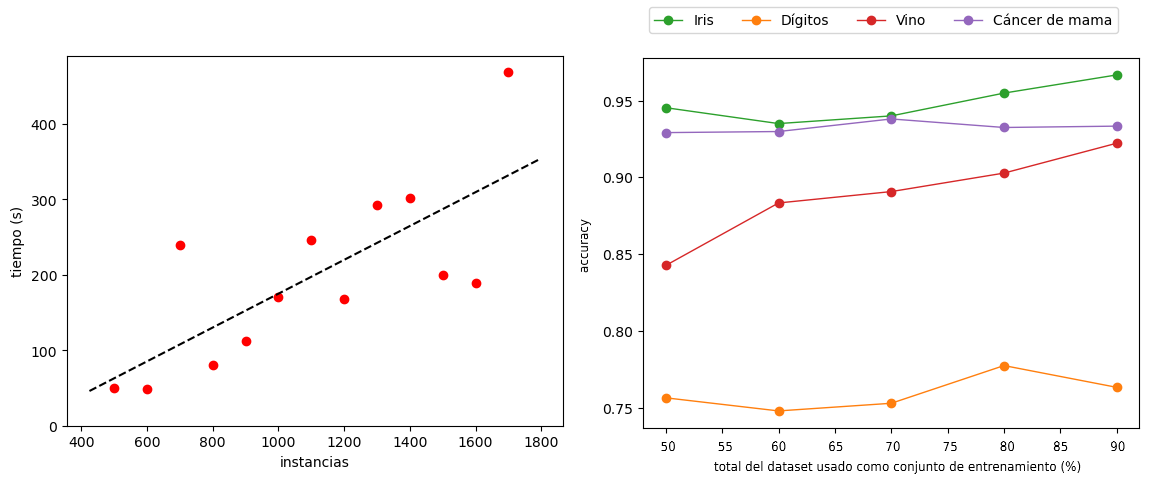
\includegraphics[scale=0.4]{../img/memoria/5_democraticco_time-percentage}
	\label{gr:dc_time-percentage}
\end{figure}
	
	\item \textbf{Tiempo de entrenamiento:} los resultados se plasman en la gráfica~\ref{gr:dc_time-percentage}. Como se puede comprobar, en este algoritmo el tiempo de entrenamiento requerido es muy superior a los anteriores y, aparentemente, no se asemeja a ninguna función estándar (los puntos están más dispersos que en otras ocasiones).
	
	\item \textbf{Datos de entrenamiento:} se muestra en la gráfica~\ref{gr:dc_time-percentage} (segundo cuadrante) la variación del \textit{score} del \textit{democratic-co} en función del porcentaje del conjunto de datos destinado al entrenamiento. En este caso la variación es menos notoria que en algoritmos anteriores para la mayoría de los \textit{datasets}, lo que puede implicar que el número de instancias etiquetadas puede ser inferior sin afectar tanto el desempeño del algoritmo.
	
	
\end{itemize} 


\subsubsection{Comparativa contra sslearn}

En el caso del \textit{democratic-co}, se ha optado por comparar la implementación propia contra sslearn~\cite{sslearnRepo}. Nuevamente, los resultados mostrados son producto de experimentos realizados mediante validación cruzada con 10 \textit{folds}, y ambos modelos han sido entrenados con los mismos $L$ y $U$ y probados con idénticos conjuntos de \textit{test}.

Como estimadores base en ambos modelos se han utilizado un \textit{naive-bayes} gaussiano, un árbol de decisión y un \textit{$k$NN} con $n = 3$, cuya implementación se encuentra disponible en la librería Scikit-learn.

\begin{figure}[h]
	\caption[\textit{Democratic-co}: comparativa contra \textit{sslearn}]{Comparativa contra sslearn para el \textit{democratic-co}. Se representa la \textit{accuracy} obtenida en cada \textit{fold} y la media de los mismos para ambos modelos.}
	\centering
	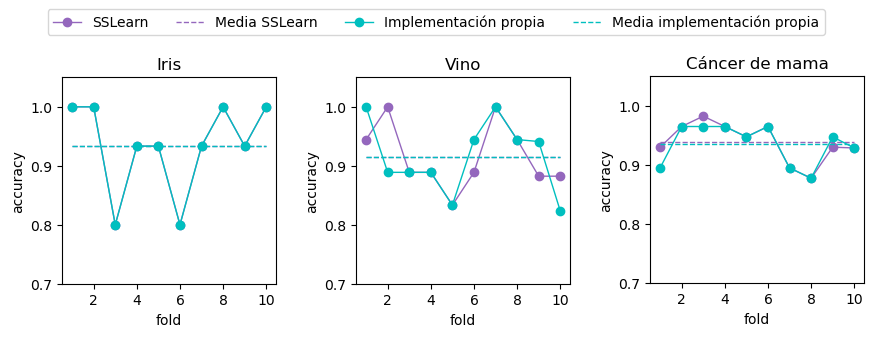
\includegraphics[scale=0.62]{../img/memoria/5_democraticco_sslearn}
	\label{gr:dc_vs_sslearn}
\end{figure}

El resultado se puede contemplar en la gráfica~\ref{gr:dc_vs_sslearn}, donde se muestra la \textit{score} obtenida en cada \textit{fold} y la media de los $10$. En el caso de Iris, la \textit{score} obtenida para cada \textit{fold} es idéntica en ambas implementaciones y, por lo tanto, la media también. El caso del conjunto de datos Vino es el que menos se asemeja, pero igualmente se ha obtenido la misma exactitud en un 60\% de las ocasiones y la media se diferencia en apenas dos centésimas. En el último \textit{dataset} binario se encuentra alguna pequeña varición en algunos \textit{folds}, pero la media obtenida es la misma.

Debido a que las pequeñas variaciones se deben a cuestiones de implementación no definidas en el pseudocódigo de Zhou y Goldman~\cite{democraticCoLearning2004original} (por ejemplo, el tratamiento de instancias duplicadas de $U$ en $L_i$), se considera que la comparativa es exitosa (el \textit{score} obtenido es idéntico en dos de los \textit{datasets} y muy similar en el otro) y el algoritmo ha sido implementado correctamente.


\section{Detección de ataques en sistemas de recomendación}
\label{sec:5_detec_ataques}
El objetivo de este apartado en el proyecto es probar nuevos métodos de aprendizaje semisupervisado aplicados a la detección de ataques en sistemas de recomendación. Para lograr este fin, se decidió, en primer lugar, reproducir el artículo original~\cite{zhou2021SemisupervisedRecommendationAttack}, que utiliza el algoritmo \textit{co-forest}. Como los autores no especifican detalles de implementación en su artículo (cómo construir perfiles de ataque, dónde encontrar bases de datos o código, etc.), se concluyó que comparar los resultados obtenidos contra los suyos es la mejor forma de determinar la correctitud del trabajo desarrollado. Para ello, se ha utilizado el \textit{dataset} MovieLens10M.

\subsection{MovieLens 10M}

MovieLens10M~\cite{groupLensDatasets} es un conjunto de datos utilizado típicamente en la investigación y desarrollo de sistemas de recomendación. Contiene 10\,000\,054 opiniones generadas por 71\,567 usuarios acerca de 10\,681 películas. Estas reseñas han sido recopiladas del servicio \textit{online} de películas MovieLens\footnote{https://movielens.org/}.

Los usuarios han sido seleccionados aleatoriamente entre los perfiles que tengan más de 20 películas valoradas y está documentado que todos son auténticos~\cite{zhou2021SemisupervisedRecommendationAttack} y pertenecen a usuarios reales. Por lo tanto, los perfiles atacantes han de ser construidos mediante programación.

\subsubsection{Creación de reseñas atacantes}
\label{sec:creacion_reseñas_atacantes}

Se han incluido tres tipos de ataques distintos: \textit{random}, \textit{average} y \textit{bandwagon}. En primer lugar, se han sintetizado las reseñas y posteriormente se han generado los vectores de características idénticamente a los perfiles verdaderos.

La metodología de construcción de las valoraciones sigue los modelos estadísticos expuestos en la sección~\ref{sec:tipos_ataques_recomendacion}. Sin embargo, se puede visualizar un resumen de los escogidos en la tabla~\ref{ataques_coforest}.

\begin{table}
\begin{centering}
	\begin{tabular}{@{}p{5em} p{6em} p{11em} p{8em}@{}}
		\toprule
		\textbf{Modelo} & $\hfil{I_S}$ & \textbf{Valoración} $\mathbf{I_F}$ &  \textbf{Valoración} $\mathbf{I_t}$\\ 
		\midrule
		Random & $\hfil\emptyset$ & Aleatoria siguiendo una distribución $\mathcal{N}(\mu,\,\sigma)$. & máxima o mínima \\
		Average & $\hfil\emptyset$ & Aleatoria siguiendo una distribución $\mathcal{N}(\mu_i,\,\sigma_i)$. & máxima o mínima\\
		Bandwagon (\textit{random}) &\centering$k$ ítems más populares & Aleatoria siguiendo una distribución $\mathcal{N}(\mu,\,\sigma)$. & máxima o mínima\\
		\bottomrule
	\end{tabular}
	\caption[Experimentación: características de ataques a detectar]{Características estadísticas de los tipos de perfiles atacantes.}
	\label{ataques_coforest}	
\end{centering}
\end{table}

Para construir las reseñas pertenecientes a un ataque del tipo \textit{random}, se ha obtenido, en primer lugar, la media de la puntuación general para todas las películas del sistema y su desviación. Los ítems de relleno han sido seleccionados aleatoriamente entre toda la base de datos (excluyendo, evidentemente, los ítems objetivo), y se ha asignado a cada uno una puntuación aleatoria siguiendo una distribución normal parametrizada por la media y desviación <<global>> del sistema. Evidentemente, esta puntuación ha sido corregida para que se encuentre entre los rangos admitidos (por ejemplo, de $0$ a $5$ estrellas). Debido a que el método de detección utilizado no necesita fechas, el campo perteneciente a la \textit{timestamp} no ha sido rellenado. Posteriormente, se ha asignado la máxima puntuación a los ítems objetivo (\textit{push attack}).

En el caso del ataque \textit{average}, el procedimiento ha sido el mismo, solo que en este caso las puntuaciones de los ítems de relleno son más representativas. En lugar de seguir una normal parametrizada por las características del sistema a nivel global, se ha calculado para cada película su media y su desviación, y se ha asignado una valoración aleatoria que sigue esta distribución. Es decir, cada ítem de relleno recibe una puntuación aleatoria que sigue una distribución normal con media la correspondiente a ese ítem en concreto, y con su respectiva desviación. En caso de que se escoja una película nunca antes valorada, la media utilizada es la media del rango (por ejemplo, 2.5 estrellas) y la desviación es $0$.

Por último, el ataque \textit{bandwagon}. Este ataque se realiza exactamente igual que el \textit{random} solo que, además, se añade un conjunto nuevo, los <<ítems seleccionados>> o $I_s$. En este caso, se escogen los $k$ ítems más populares de la base de datos (se entiende por más <<popular>> aquel ítem que posea más valoraciones). Evidentemente, este conjunto se excluye (además de los ítems objetivo) a la hora de escoger los ítems de relleno. La valoración asignada a $I_s$ ha sido o bien la máxima, o bien la mínima (en función de su nota media).

\subsubsection{Generación de conjuntos de entrenamiento y \textit{test}. Parámetros.}

Para generar el conjunto de entrenamiento, se ha utilizado el mismo proceso que el descrito en el \textit{paper} de Zhou y Duan~\cite{zhou2021SemisupervisedRecommendationAttack}. La distribución de los datos utilizados se muestra en la tabla~\ref{tbl:entrenamiento_ML10M}.

En primer lugar, se han seleccionado 1\,000 perfiles aleatorios verdaderos y se han extraído sus vectores de características como se ha indicado previamente en la sección~\ref{sec:vectores_catacterísticas_ataquesisrec}. Posteriormente, se han generado reseñas para perfiles de atacantes, y se han extraído sus vectores.

\begin{table}
	\begin{centering}
		\begin{tabular}{@{} p{9em} p{7em} p{3em} p{3em} p{3em} p{3em} @{}}
			\toprule
			\multirow{2}{*}{\hfil \textbf{Tipo}} & \multirow{2}{*}{\hfil \textbf{Número}} & \multicolumn{4}{c}{\hfil \textbf{Tamaño del relleno}} \\ \cmidrule{3-6}
			&\hfil   &\hfil \textbf{1\%} &\hfil \textbf{3\%} & \hfil \textbf{5\%} & \hfil \textbf{10\%}\\ 
			\toprule
			Genuino &1000&\hfil -	& \hfil -  & \hfil - & \hfil -\\
			\textit{Random attack} &-	&\hfil 10 & \hfil 10	&  \hfil 10 & \hfil 10\\
			\textit{Average attack} &-	& \hfil 10 & \hfil 10 & \hfil 10 & \hfil 10 \\
			\textit{Bandwagon attack} &- & \hfil 10 & \hfil 10 & \hfil 10 & \hfil10 \\
			\\ \bottomrule
		\end{tabular}
	\end{centering}
	\caption[Sistemas de recomendación: descripción de los conjuntos]{Número y distribución del conjunto de entrenamiento.}
	\label{tbl:entrenamiento_ML10M}	
\end{table}

En cuanto al conjunto de test, se han generado $10$ conjuntos distintos para garantizar que los resultados de los experimentos no son fruto de una partición concreta de los datos, sino media de una cantidad aceptable. Para ello, se han realizado ficheros \texttt{.csv} para distintos porcentajes de tamaño de ataque ($1\%, 2\%, 5\%$ y $10\%$) y tamaño de relleno ($1\%, 3\%, 5\%$ y $10\%$) de los atacantes. El número de perfiles verdaderos en cada conjunto de \textit{test} equivale a $1000$ (y son excluyentes entre ellos y respecto al conjunto de entrenamiento).

En cuanto a los parámetros del algoritmo, se han establecido los mismos que en el \textit{paper} de Zhou y Duan~\cite{zhou2021SemisupervisedRecommendationAttack}. El tamaño de ventana ($J$) se ha establecido a 40 y el porcentaje de etiquetas en el conjunto de entrenamiento ($d$) equivale al $30\%$. Como el \textit{paper} no indica qué hacer en el caso del \textit{bandwagon}, se ha decidido que el número de ítems relevantes a evaluar ($k$) es 30. En cuanto al \textit{co-forest}, el umbral de confianza $\theta$ se ha fijado a $0$.$75$ y el número de árboles ($n$) utilizado es 6.

Cabe destacar que, debido a que es escaso el número de instancias positivas, se ha decidido utilizar como curva para calcular las AUC la curva \textit{precision-recall} (en lugar de la curva ROC).

\subsubsection{Resultados}

Los resultados se han desglosado en función del tipo de perfiles atacantes inyectados. Se ilustran en las respectivas gráficas: \textit{random attack}~\ref{5_random_attack}, \textit{average attack}~\ref{5_average_attack} y \textit{bandwagon attack}~\ref{5_bandwagon_attack}.

En la leyenda se puede comprobar que se han utilizado distintos algoritmos de ML. Para comparar el \textit{co-forest} con el \textit{random forest}, se han utilizado dos versiones de este mismo (etiquetadas como <<RF-A>> y <<RF-L>>). RF-A es un \textit{random forest} que ha sido entrenado con el conjunto de entrenamiento al completo (es decir, con el $100\%$ de las etiquetas disponibles). RF-L también es un \textit{random forest}, pero la diferencia reside en que, en este caso, únicamente se han utilizado un $30\%$ de las etiquetas disponibles en su entrenamiento (las mismas que se proporcionan al \textit{co-forest}). Este \textit{ensemble} permite deducir si el \textit{co-forest} (algoritmo semisupervisado) resulta verdaderamente útil en una situación de escasez de etiquetas, o si por el contrario es mejor utilizar la versión supervisada. Por último, también se ha incluído un \textit{tri-training} que utiliza como estimadores base un \textit{naive-bayes} gaussiano, un árbol de decisión y un \textit{$k$NN}.

\begin{figure}[h]
	\caption[\textit{Random attack}: detección.]{Gráfica que representa la detección de perfiles que utilizan \textit{random attack} en el \textit{dataset} MovieLens10M.}
	\centering
	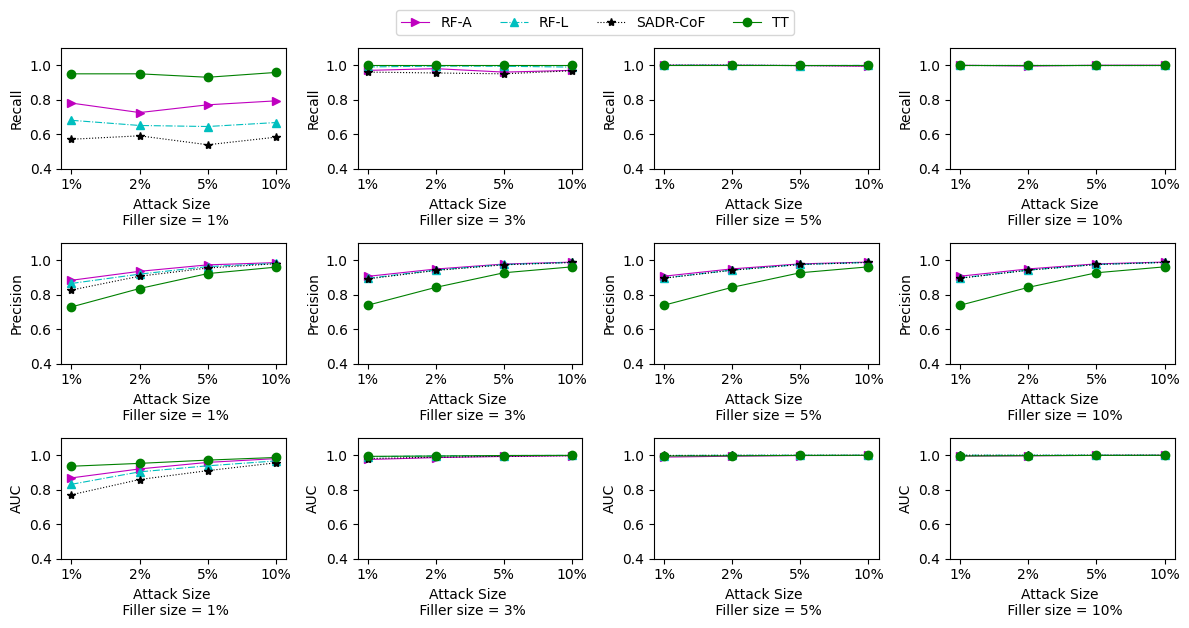
\includegraphics[scale=0.45]{../img/memoria/5_resultados_random_attack}
	\label{5_random_attack}
\end{figure}

\begin{figure}[h]
	\caption[\textit{Average attack}: detección.]{Gráfica que representa la detección de perfiles que utilizan \textit{average attack} en el \textit{dataset} MovieLens10M.}
	\centering
	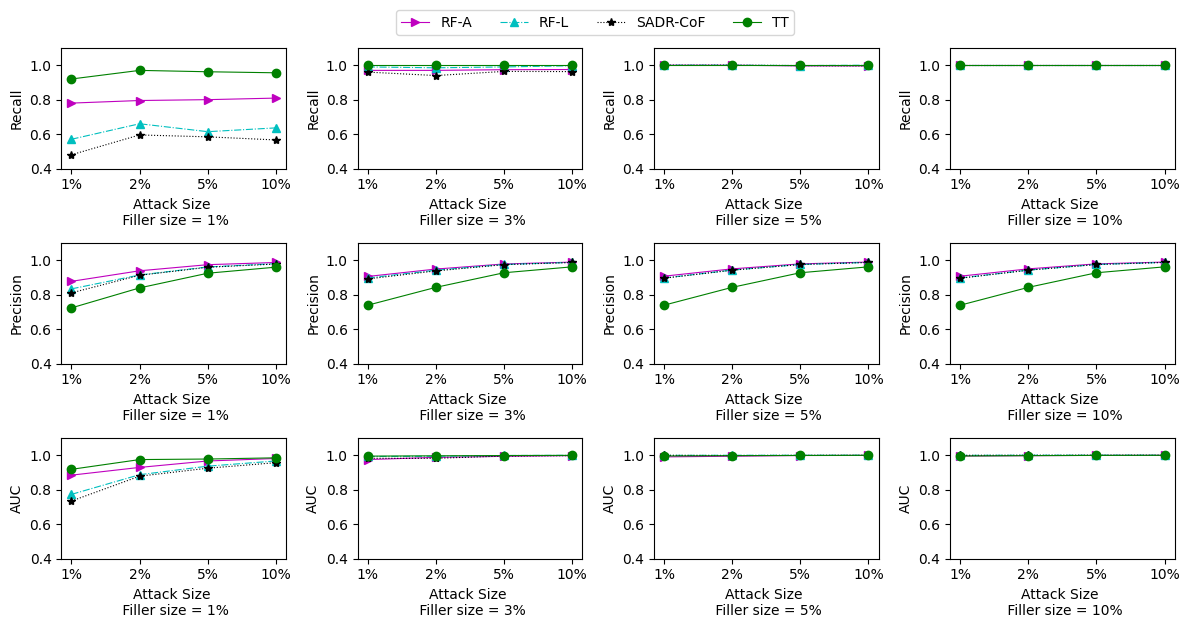
\includegraphics[scale=0.45]{../img/memoria/5_resultados_average_attack}
	\label{5_average_attack}
\end{figure}

\begin{figure}[h]
	\caption[\textit{Bandwagon attack}: detección.]{Gráfica que representa la detección de perfiles que utilizan \textit{bandwagon attack} en el \textit{dataset} MovieLens10M.}
	\centering
	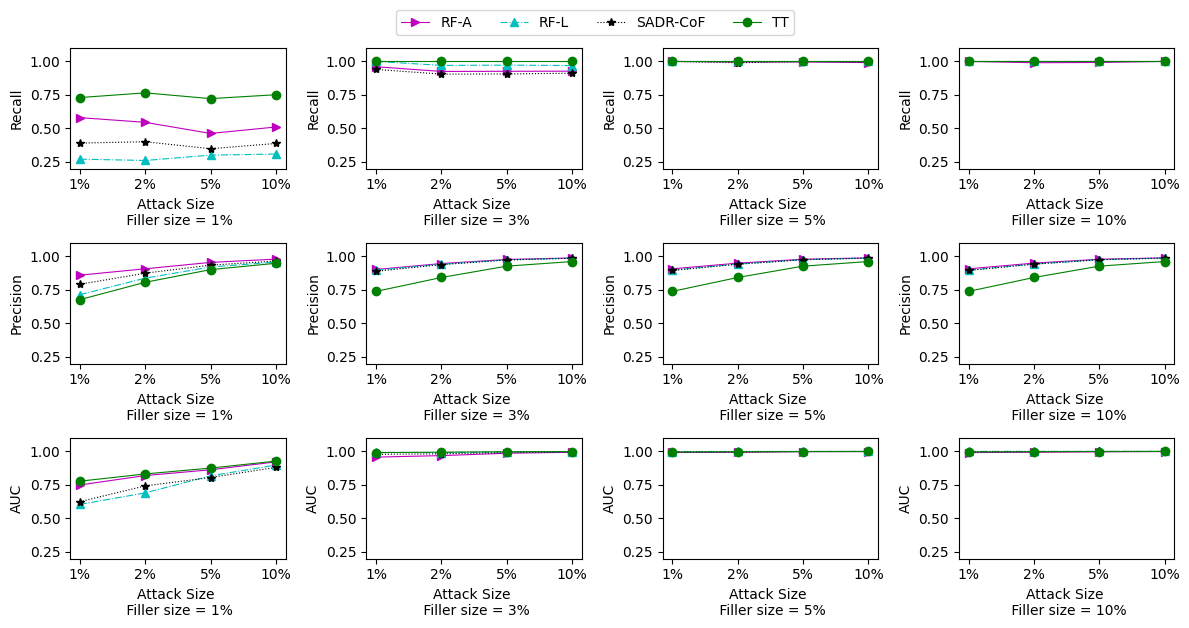
\includegraphics[scale=0.45]{../img/memoria/5_resultados_bandwagon_attack}
	\label{5_bandwagon_attack}
\end{figure}

\subsubsection{Discusión de los resultados}

Puede parecer que los resultados son muy satisfactorios debido a que, en situaciones en las que el \textit{filler size} del atacante es mayor o igual que el $3\%$, el \textit{recall} (es decir, la cantidad de instancias positivas que se encuentran) para la mayoría de los algoritmos es muy alto y la precisión (de las instancias que se clasifican como positivas, cuántas lo son realmente) es generalmente buena (exceptuando tal vez, la del \textit{tri-training}, lo que es lógico porque también posee un \textit{recall} mayor).

Sin embargo, una de las fases del ciclo de vida del ML es el preanálisis de datos. Si se observa con detenimiento el \textit{dataset}, se puede comprobar que la media del \textit{filler size} de los usuarios genuinos es aproximadamente de un 1.34$\%$ y que únicamente un 10$\%$ de los usuarios tiene un \textit{filler size} superior al 3$\%$. Por ello y teniendo en cuenta que para cada conjunto (ya sea de entrenamiento o de \textit{test}) se selecciona aleatoriamente un 1.45\% del total los usuarios genuinos, es muy probable que esté formado por perfiles con un \textit{filler size} inferior al 3$\%$. Por lo tanto, la única <<columna>> verdaderamente significativa es la primera, y como se puede comprobar los resultados no son buenos. En otras palabras, es muy probable que el \textit{recall} sea tan bueno en la mayoría de los casos porque los perfiles inyectados tienen un número de valoraciones muy superior a los perfiles genuinos, no porque el método de extracción sea relevante y significativo.

Adicionalmente, se piensa que el método de extracción de vectores de características no es muy adecuado. El hecho de que se aplique directamente en bases de datos sin ningún tipo de ordenación implica que tiene que existir alguna relación subyacente en el orden <<por defecto>> de los datos y el comportamiento de los usuarios, lo que es una suposición que no puede extrapolarse a todos los conjuntos de datos. Si la base de datos estuviese, por ejemplo, ordenada por popularidad, sería natural que los usuarios votasen más en las primeras ventanas. Si estuviese ordenada por fechas, podría existir una relación entre la edad del usuario y las ventanas en las que vota (películas de su <<época>>). Sin embargo, al no existir ningún tipo de orden, es una hipótesis demasiado general para ser asumida. Por ello, se ha decidido cerrar esta línea de investigación.


\section{Detección de \textit{phishing}}
\label{sec:5_phishing}
Se detalla a continuación el proceso seguido en las distintas fases relacionadas con la experimentación.

\subsection{Extracción de las URL del \textit{dataset}}

\begin{table}
	\begin{centering}
		\begin{tabular}{@{} p{10em} p{6em} p{6em}@{}}
			\toprule
			\textbf{\textit{Dataset}} &\raggedleft\textbf{Instancias} &\hfil\textbf{Categoría} \\ \midrule
			\textit{Phishtank} & \raggedleft 1\,528 &\hfil \textit{Phishing}\\
			\textit{Openphish} & \raggedleft 613 &\hfil \textit{Phishing}\\
			Alexa & \raggedleft 1\,600 &\hfil Genuino\\
			Plataforma de pago & \raggedleft 66 &\hfil Genuino\\
			Páginas de banca & \raggedleft 50 &\hfil Genuino\\
			\bottomrule
		\end{tabular}
		\caption[\textit{Phishing}: descripción del \textit{dataset}]{\textit{Dataset} de \textit{phishing}.}
		\label{tbl:dataset_phishing}	
	\end{centering}
\end{table}

Para extraer los vectores de características, en este caso, se necesita extraer el \texttt{html} de distintas páginas web (tanto verdaderas como de \textit{phishing}) mediante peticiones de código, por lo que se necesita conocer su dirección. Para garantizar el anonimato en las peticiones que se realizan a páginas de \textit{phishing}, se han utilizado \textit{proxies} con un protocolo SOCKS5. Para levantarlos, se ha utilizado un \textit{script} de implementación propia descrito en la sección~\ref{sec:script_tor}.

Se ha intentado replicar el \textit{dataset} (procedencia y número) utilizado en el \textit{paper} de Jain y Gupta~\cite{featuresPhishing2018Gupta}, pero muchos de los enlaces facilitados no están disponibles actualmente. Por ello, se han buscado alternativas y el resultado final se muestra en la tabla~\ref{tbl:dataset_phishing}.

En el caso de Phish Tank, la base de datos sigue disponible y es accesible en su página web~\cite{phishTankDB}. Debido a que se actualiza a diario, se recupera mediante una petición \textit{get}, aunque se han tenido dificultades (solucionadas utilizando \textit{proxies} y los \textit{headers} adecuados) debido a que el sitio tiende a bloquear si se hacen unas pocas peticiones seguidas. También sigue accesible la base de Open Phish~\cite{openFishDB}, aunque en este caso el número máximo de instancias obtenibles gratuitamente está limitado a 500 y se puede encontrar en un fichero en su página web~\cite{openFishFile}. Debido a que también se actualiza periódicamente, se recupera en peticiones mediante código.

Los sitios legítimos se han extraído del \textit{top} 1 millón páginas visitadas mediante Alexa\footnote{\textit{Top} extraído de \url{https://www.expireddomains.net/alexa-top-websites/} debido a que Amazon está realizando reformas en el servicio.}, del \textit{top} de plataformas de pago disponibles y de algunos de los sitios de banca más populares. En el caso de los enlaces genuinos, ninguna de las direcciones facilitadas en el \textit{paper} original está disponible. Por ello, los sitios más consultados en Alexa se han obtenido de Expired domains~\cite{AlexaTopWebsites}, las plataformas de pago más comunes de Shopify~\cite{paymentGatewaysWebsites} y los sitios bancarios, al igual que en el \textit{paper} original, de Similar Web~\cite{banksitesTop} (solo que el número está limitado a 50). Debido a que los enlaces facilitados por estas plataformas no contienen protocolo, se ha generado un \textit{script} auxiliar que encuentra el correspondiente y filtra aquellas páginas en inglés y español (no se ha utilizado el \textit{header} para realizar esta tarea porque no se incluye en la librería de Python, por lo que se ha analizado el lenguaje).




